% -*-mode: latex; coding: utf-8-unix -*-
\documentclass[11pt]{article}
\usepackage[utf8]{inputenc}
%
% user-modifiable options
%
\usepackage{leading} \leading{6mm} % extra space between lines

% \usepackage[francais,UKenglish]{babel}    % last one is default language
\usepackage[a4paper]{geometry}
% \usepackage{lmodern} %% Vector fonts
%
% Font and appearance: do not change
%
% \usepackage{aeguill} %% French guillemets with T1
\usepackage{amsfonts,amsmath,amssymb} %% Additional math chars
\usepackage{eurosym} %% \euro symbol
\usepackage[T1]{fontenc} %% Vector fonts
\usepackage[babel]{microtype} % load microtype after babel, inputenc, and font-changing packages
% \usepackage{flushend}	% balanced last page in 2-col formatting
%
% Useful packages.  Optional.
%
\usepackage{graphicx}
\usepackage[numbers,square,sort&compress]{natbib}
\usepackage[defblank]{paralist} % inline lists
\usepackage{parskip} \parskip=1ex plus 5pt minus 1pt \parindent=4ex %% indent paragraphs
\usepackage[obeyspaces]{url} \urlstyle{sf} %% URLs 
% \usepackage[verbatim]{svn-multi}
\usepackage{xcolor}
\usepackage{xspace}
\usepackage{hyperref}  %% hyperlinks in PDF (must be last package loaded)
    \newcommand{\hhref}[2]{\href{#2}{#1}} %{text}{URL}


\newcommand\todo[1]{\textcolor{blue}{(TODO: #1)}}
\newcommand{\commentaire}[2][fromWhom?]{{
  \color{magenta}{\bfseries\sffamily\scriptsize$\triangleright$(#1:) #2$\triangleleft$}
}}

\begin{document}
\author{
  Saalik Hatia\\
  \texttt{Sorbonne Université}
  }
\title{Specification of a TCC database}


\date\today
\maketitle
% \tableofcontents



\section{Problem Statement}
\label{sec:problem-statement}
The geo-distributed database system Antidote persists its
updates in a log.
To recover after a crash, or to materialize a version of interest,
requires to read and to (re-)execute all the corresponding operations
from the journal from the initial state.
As a database ages, this takes longer and longer.

The aim of this research is to speed this up by adding a checkpointing
mechanism.
Initializing from a recent checkpoint requires to re-execute only
the operations after the checkpoint, which can be much faster.
Once a full-system checkpoint exists, the preceding part of the log can
be truncated if desired.

Journaling, materializing, checkpointing and journal truncation are
well-known mechanisms.
However, their interplay is known to be tricky; this will be even more
challenging in Antidote, because of its complex geo-distributed and
sharded structure, and because of its partially-ordered consistency
model.

The aim of this research is to specify rigorously, and to implement
correctly and efficiently, a safe journaling, materializing,
checkpointing and truncation mechanism for Antidote.
This includes the following partial objectives:
\begin{compactitem}
\item
  To specify the structures of interest, i.e., distributed journal,
  materialization cache, and checkpoint store.
\item
  To specify the concepts of consistent cut, snapshot, object version,
  checkpoint, and to identify the consistent cuts that are important for
  correctness and performance.
\item
  To specify rigorously the invariants that link the above structures
  together.
\item
  To identify the actors of interest and their methods: transaction
  coordinator, version cache, journal manager, checkpoint manager, etc.
\item
  To specify the pre-, post-, rely- and guarantee-conditions of these
  methods.
\item
  To implement (first in pseudocode, ultimately in running code) these
  methods.
\item
  To show that the implemented methods satisfy their specification.
\end{compactitem}
\section{Background and notation}
\label{sec:background}
The Antidote database is geo-distributed across a number of Data Centers
(DCs).
Each DC is strongly consistent; however, updates can originate
concurrently at any DC under the Transactional Causal Consistency model.

\subsection{Data Centers and shards}
\label{sec:dc-shards}
Antidote supports concurrent updates occurring in geo-distributed,
highly-available DCs; each DC originates its own set of updates.
In turn, a DC is partitioned into non-overlapping storage servers called
shards, coordinated by Transaction Coordinators.\ref{fig:architecture}
Thus, the journal is not a single sequential data structure, but is
logically the union of a number of sequential \emph{journal streams},
one per shard per DC\@.
Furthermore, a stream originating in some shard in some DC is replicated
to the same shard in all other DCs.%
%
\footnote{
%
  We ignore here the fact that a shard is itself replicated in its DC
  for fault tolerance, because this does not change the fact that each
  journal stream is sequential.
}
%

Zooming into a given shard at a given DC, the former contains a \emph{local}
journal stream that logs the updates to this shard originating from the latter,
and a set of remote journal streams, each one replicating the
updates to this same shard at some other DC\@.
%
\footnote{
  In this document we ignore the possibility of adding additionnal shards 
  and/or DCs. 
}

\begin{figure}[tp]
  \centering
  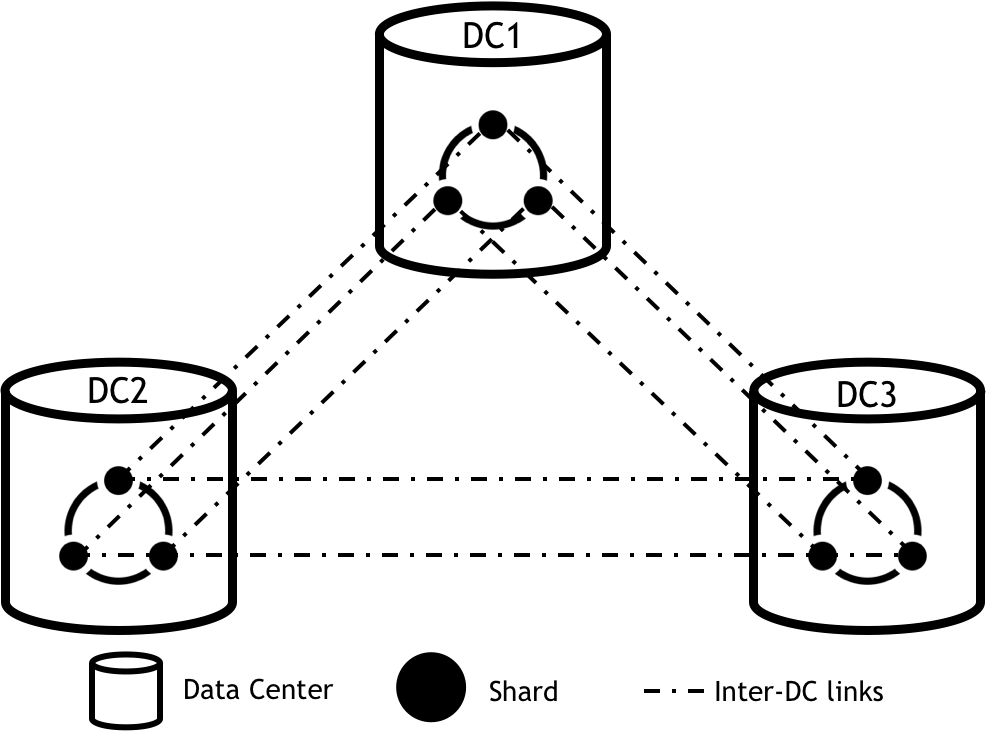
\includegraphics[width=0.75\textwidth]{figures/datacentres.png}
  \caption{Overall architecture of Antidote}
  \label{fig:architecture}
\end{figure}

\begin{figure}[tp]
  \centering
  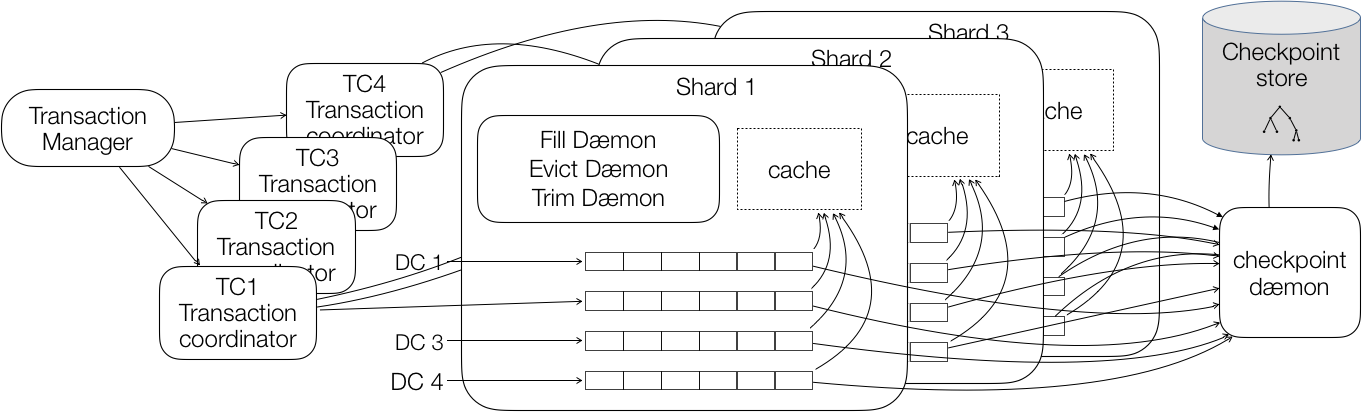
\includegraphics[width=1\textwidth]{figures/insidedc.png}
  \caption{Inside a DC. The Transaction Manager supervises Transaction Coordinators that handle all the client transactions. Every shard has a Cache, a Journal, and three daemons with a specific role. Connected to them is a Checkpoint Daemon that creates checkpoints and stores them into a Checkpoint Store.}
  \label{fig:insidedc}
\end{figure}

\subsection{Transactional Causal Consistency}
\label{sec:tcc}

Another source of complexity is the Transactional Causal Consistency
(TCC) model.
Each DC is logically sequential, based on a variant of Snapshot
Isolation.
However, two DCs may update the database concurrently, and updates are
related by the \emph{happened-before} partial order (sometimes called
causal order).

To keep track of happened-before, Antidote uses vector
timestamps with one entry per DC\@.
Every event in the database is tagged by the corresponding vector
timestamp.
A \emph{consistent vector timestamp} (CVT) marks a \emph{transactionally- and
causally-consistent cut}.
This means that, if a CVT contains some update $u$, then it also contains all
updates in the same transaction as $u$, as well as those that
happened-before $u$. 
The snapshot time of a transaction is called its \emph{dependency
CVT}, and its output is identified by its \emph{commit CVT}.

Recall that a given DC-shard has a local journal stream and one journal
stream per remote DC\@.
Similarly, a CVT has a timestamp per DC\@.
We can now map each entry in a CVT (for some DC) to the prefix of the
journal stream (of the same DC) that happened-before it.
This forms a \emph{transactionally- and causally-consistent snapshot}.


\subsection{Journal structure}
\label{sec:journal}

The events that impact the state of the store are persisted in a log, called the
Journal herein. 
The Journal constitutes the ground truth of the database state. 
The Journal is logically composed of a number of sequential streams, each of
which records the events originating from a given shard. 
A shard’s Journal stream is replicated to its counterparts at all other DCs. 

\subsection{Records}
\label{sec:record}

The events recorded in the Journal are called Records.
They contain different types of information. 
It can be system information(such as checkpoint operations), transaction
operations (such as commit message) or operations on an object.
These last operations are essential to the integrity of the database.
The loss of a single record means that all the objects that are materialized
afterward are incorrect.
Each of these records contains these entries:
\begin{compactitem}
  \item \textbf{Log Sequence Number (LSN):} A unique monotonically increasing 
  sequence number
  \item \textbf{Timestamp}: Real-time timestamp 
  \item \textbf{TransactionID:} a transaction identifier 
  \item \textbf{Type:} system operation, transaction operation
\end{compactitem}
Depending on the type of the operation the following information is included
in the record:
\begin{compactitem}
  \item \textbf{Key:} reffered object key
  \item \textbf{Operation:} referred object and its arguments or the system 
  \item \textbf{Dependency:} CVT of the snapshot the transaction is reading from
  \item \textbf{ListOfParticipants:} participants in a given transaction
  \item \textbf{CommitTime:} commit time of a transaction
\end{compactitem}

These are the different Type of operation:

\begin{compactitem}
\item \textbf{Begin:} system record that marks the beginning of a
transaction. 
It contains the Timestamp, TransactionID, Type, followed by the Dependency.
This record is written once per transaction to each shard
participating.
\item \textbf{Prepare:} system record that is written by shards during the two-phase commit. 
It contains the Timestamp, TransactionID, Type, followed by the ListOfParticipants.
The Timestamp in this context is the clock proposed by the shard as the commit time.
\item \textbf{Commit:} system record that contains the commit time sent by the coordinator
to the shards once the two phase protocol is finished.
It contains the Timestamp, TransactionID, Type, CommitTime.
The commit time is sent to the shard by the transaction Coordinator.
\item \textbf{Abort:} system record that marks the abortion of a transaction.
It contains the Timestamp, TransactionID, Type, ListOfParticipants.
\item \textbf{Update:} transaction record containing the update operation on a given
object.
It contains Timestamp, TransactionID, Type, Key, Operation.
\end{compactitem}


\subsection{Checkpoint store}
\label{sec:checkpoint-store}

In this design we persist periodically materialized versions of objects, called
checkpoints in a store called the Checkpoint Store.  
In the worst case after a crash, all volatile state has been lost, the current
state of an object can be computed by: (1) loading the most recent checkpoint
into memory, (2) reading updates that postdate the checkpoint from the journal,
(3) applying those updates to the in-memory state.

Once an object has been checkpointed, any earlier journal record that is part of 
the checkpoint for that object is irrelevant. 
Checkpoints are created from a causally-consistent cut called Checkpoint Time
(CT) (Section \ref{sec:checkpoint-time}) to ensure that there are no consistency
anomalies in the checkpoint.
Once all the objects in a CT have been checkpointed, then the corresponding
prefix of the journal can be truncated. 

%%%%%%%%%%%%%%%%%%%%%%%%%%%%%%%%%%%%%%%
\section{Consistent cuts of interest}
\label{sec:tcc-cuts}
The causal ordering of events implies that their vector timestamps are
ordered in the same way:
If Event~1 is causally-before Event~2, their vector timestamps
\emph{vt1} and \emph{vt2} are such that 
\emph{vc1 $<$ vc2}.
Note that the converse is not true in Antidote.
The timestamps of two
concurrent events may be either incomparable or arbitrarily ordered (a
timestamp is a safe approximation).

The order between vector timestamps \emph{vt1} and \emph{vt2} is defined
as followed:
\begin{compactitem}
\item
  \emph{vt1 = vt2} if every entry of \emph{vt1} is equal to the
  corresponding entry of \emph{vt2}.
  They represent the same event.
\item
  \emph{vt1 $\le$ vt2} if every entry of \emph{vt1} is less or equal to
  the corresponding entry of \emph{vt2}.
\item
  \emph{vt1 $<$ vt2} if \emph{vt1 $\le$ vt2} and \emph{vt1 $\neq$ vt2}.
  Event~1 being causally before Event~2 implies \emph{vt1 $<$ vt2}, but the converse
  is not guaranteed.
\item
  \emph{vt1} is incomparable to \emph{vt2} if \emph{vt1 $\neg\le$ vt2
    $\land$ vt1 $\neg\le$ vt2}.
  There is some entry in \emph{vt1} that is lower than the
  corresponding entry in \emph{vt2}, and vice-versa.
  Events~1 and~2 are necessarily concurrent, but the converse is not true;
  that is, if two vector timestamps are incomparable, this does not guarantee
  that the corresponding events are concurrent.
\end{compactitem}
A vector timestamp represents a \emph{cut} or time of the data store.
We are interested only in \emph{CVTs} as they have properties that are 
useful for maintaining information about the database.
%%%%%%%%%%%%%%%%%%%%%%%%%%%%%%%%%%%%%%%

% \commentaire[Saalik]{The idea here is to start with the checkpoint time and 
% build up from there}

\subsection{Checkpoint Time (CT)}
\label{sec:checkpoint-time}
Every time a checkpoint is created, we persist the operation in the Journal
(Section \ref{sec:journal}).

The variable \emph{Checkpoint Time} designates the \emph{oldest} available
checkpoint, i.e., lowest \emph{CVT} that includes, for every object, a
checkpoint whose state includes all the update records committed at any time
$\le \mathit{Checkpoint Time}$.
State prior to \emph{CT} cannot be safely recovered.

If the checkpoint store does not support versioning (i.e., each object
has a single version), then there is a single checkpoint, identified by
\emph{Checkpoint Time}.
Initially, \emph{Checkpoint Time = $-\infty$}, implying that the journal
cannot be trimmed.

Note that, while recovering from \emph{CT} is safe, typically recovery will
proceed from the \emph{most recent} available checkpoint for performance
reasons.
To save space, a system typically stores only a few numbers of checkpoints,
preferably only one. 

%%%%%%%%%%%%%%%%%%%%%%%%%%%%%%%%%%%%%%%

\subsection{DC-Wide Causal Safe Point (DCSf)}
\label{sec:dcsf}
Each shard in a DC is replicated to all other DCs.
All updates that originate in some DC are sent asynchronously to the
corresponding shard in other DCs.
Although the shard-to-shard connection is FIFO, the storage state of
different shards in the same DC is not causally consistent.
Without extra care, a transaction that reads from multiple shards might
be unsafe, or has to wait, because a shard is missing updates with
respect to another.

The Cure protocol \cite{rep:pro:sh182} is what ensures the TCC properties.
Cure has two main objectives:
\begin{compactenum}[(1)]
\item 
  To ensure that transactions in a DC commit atomically, and in a
  total order across all shards of that DC\@.
  It uses the Clock-SI design for this purpose
  \cite{rep:pan:1723}).
\item
  To ensure that that updates are observed in a causally-consistent
  order within a DC\@.
  To this effect, each shard continuously computes a safe lower bound
  for that DC, called its DC-Wide Causal Safe Point (DCSf).%
\footnote{
  % 
  Called the Global Stable Snapshot (GSS) in the Cure paper
  \cite{rep:pro:sh182}.
}
  The DCSf is a \emph{CVT} across all shards of the DC that is
  \emph{causally safe}, i.e., the corresponding updates, and their causal
  predecessors, have been received and persisted by all shards of this DC.
  States that are above the DCSf are not \emph{visible}.
  A transaction whose snapshot time is not earlier than the DCSf would
  be blocked until the DCSf advances beyond it.
\end{compactenum}
%%%%%%%%%%%%%%%%%%%%%%%%%%%%%%%%%%%%%%%

\subsection{Global Causal Stable Point (GCSt)}
\label{sec:causal-stable-snapshot}

In our new design, we will also leverage the concept of a
\emph{Global Causal Stable point} (GCSt).
A GCSt is a state where all concurrent operations have been received and
resolved.
Formally, any updates that are delivered after the GCSt is computed will
have a higher timestamp than the GCSt
\cite[Definition~5.1]{app:rep:1800}.
To simplify the logic, we assume that successive computations of a GCSt
at some shard are monotonically non-decreasing (this is always
possible).
To compute the GCSt each shard shares its DCSf periodically with their
counterparts in other DCs. 
Using this information every shard computes the minimal point of advancement of
all the DCs. 

To store some state that is earlier than the GCSt, means we can use its
sequential representation, avoiding any concurrency-related metadata such as
vector clocks or tombstones.
The transitions between successive GCSt's can be explained as sequential
updates.
This makes the representation simpler and more compact and enable the 
use of any sequential database as a checkpoint store.
For instance, both Add-Wins and Remove-Wins sets reduce to classical
sequential sets, and RGA reduces to a classical list.

One issue with GCSt is that it makes progress only when every single DC
is available.
It stops advancing as soon as any single DC does not regularly communicate its
metadata.

\subsection{Min-Dependency and Max-Committed}
\label{sec:dep-commit}
In order to satisfy the properties of checkpoints, the DCSf and the GCSt we keep
track of all the dependencies of running transactions but also all the commit
times of finished transactions. 
Among those we single out those who are the most important.

The first one is called Min-Dependency it represents the oldest snapshot any
running transaction is reading from. 
Because one key property of the checkpoints is that they are sequentially
consistent, there should be no in-flight transactions at Checkpoint-Time.
To ensure this property holds true Min-Dependency is used to track the point
beyond which sequentiality is not guaranteed.
When a transaction is finished, committed or aborted, the Min-Dependency
advances to the next Dependency. 
One issue is that until a transaction is running Min-Dependency
will not advance and consequently snapshotting will be paused.

The second one called Max-Committed is the last commit time recorded in the
Journal.
It is used to control the advancement of the DCSf making sure that a new
transaction does not read unsafe updates.
Every time a transaction commits, its commit time become the new Max-Committed.
Similarly to Min-Dependency, if no transaction commits than Max-Committed does
not advances and the DCSf is blocked up until that point.

\subsection{Low and High}
\label{sec:low-high}
To represent the persistent portion of the log we use Low and High. 
With \emph{Low} representing the lower bound and \emph{High} the higher
bound.
Records that precedes \emph{Low} may be deleted and records that postdates
\emph{High} might be volatile.

\subsection{Invariants}
\label{sec:cuts-invariants}

The overarching goal of this work is to have no perceivable loss of information,
meaning records that have not been checkpointed must not be deleted.
Hence, our first invariant $\mathit{Low} \le \mathit{Checkpoint Time}$.
One key property of checkpoints is that they should be sequentially consistent
and stable across all DCs.
Hence, the second and third invariant $\mathit{Checkpoint Time} \le
\mathit{GCSt}$ and $\mathit{Checkpoint Time} \le \mathit{Min-Dependency}$.
By construction the GCSt is computed using all the DCSf across all the DCs so
this gives us the following invariant $\mathit{GCSt} \le
\mathit{DCSf}$. 
DCSf represents the point of safety in a DC using shared information between
shards about their registered \emph{commit times} therefore $\mathit{DCSf} \le
\mathit{Max-Committed}$. 
These relations control the behavior of each shard \ref{fig:system-vts}

\begin{figure}[tp]
  \centering
  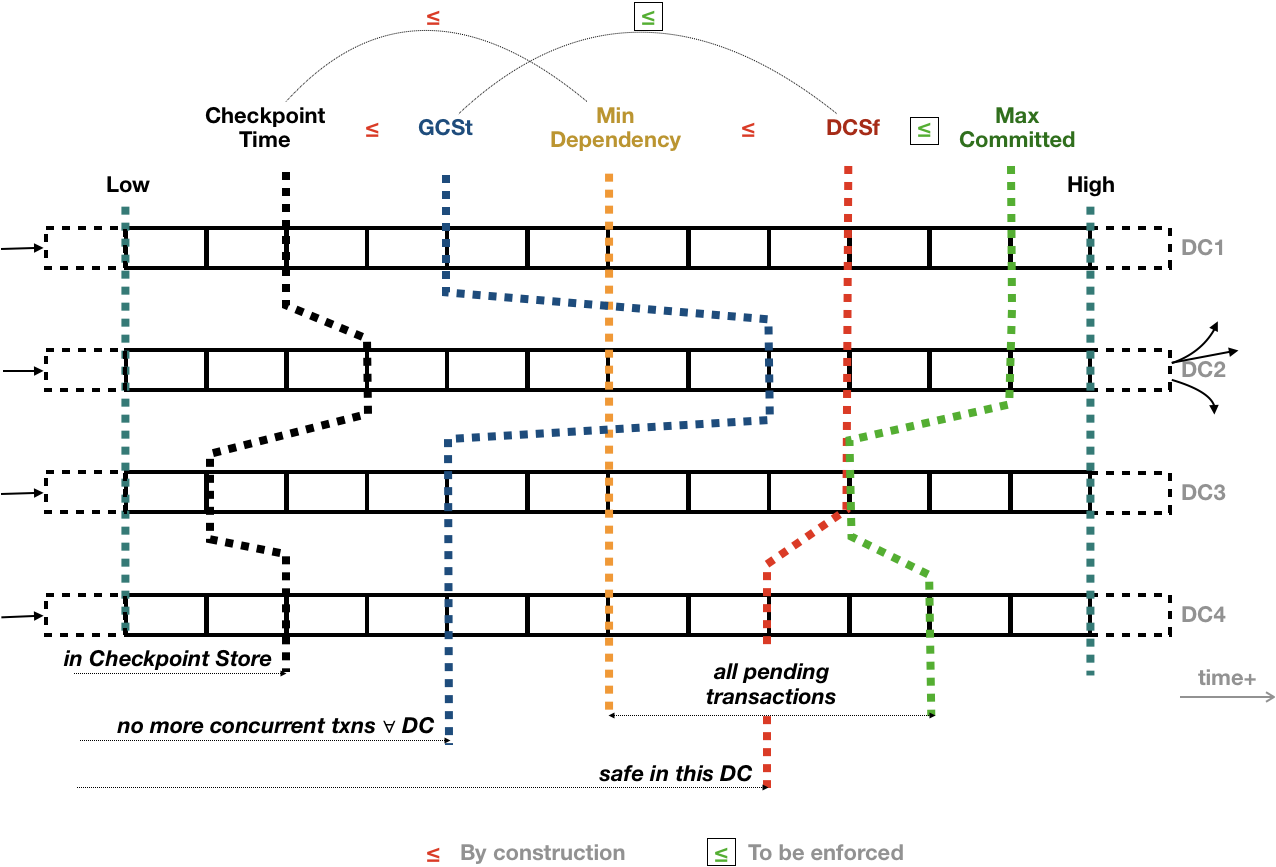
\includegraphics[width=\textwidth]{figures/cvts.png}
  \caption{%
    Relevant system states and their relations (for a given
    shard, at a given DC).
    Each horizontal tape (one per DC) depicts a journal stream for
    this shard.
    Each vertical line depicts a cut of interest and its
    vector timestamp.
    Over time, each journal stream grows to the right (and is
    trimmed to the left), and each state of interest advances
    monotonically to the right.
    As this happens, the causal precedence invariants, denoted
    $\le$, must be maintained.
  }
  \label{fig:system-vts}
\end{figure}


\section{Cache}
\label{sec:cache}

The cache maintains materialized versions of objects that are currently in use. 
An entry in the cache is identified by a pair \emph{(k,c)} where
\emph{key} is the key of the object, and \emph{c} is the commit timestamp of the
version. 
Each shard maintains its own cache.

\subsection{Object-version descriptors}
\label{sec:objects}

The system maintains the following information about an object's version
in an object-version (\emph{entry (e)}):
\begin{compactitem}
\item
  \emph{key (k)} is the key of the object.
\item
  \emph{commit (c)} is the commit vector timestamp of the transaction
  this object is materialized from.
  An uninitialized object-version has a vector timestamp of $-\infty$.
\item
\emph{presence (p)}: the present bit, it is true when the descriptor is
significant. 
Otherwise, it must be ignored.
\item
  \emph{valid (v)} is a vector timestamp for which the object has
  not been updated.
  In other words, it is known that there exist no committed
  updates between \emph{commit} and \emph{valid}.
  Equivalently, this version is part of all snapshots between these two
  values.
\item
  \emph{used (z)} a bit that indicates that this version has been recently been
  used; useful for cache management.
\item
  \emph{blob (b)} is a pointer to the materialized value of the object (if
  any), either in memory or on checkpoint store.
  The system does not interpret the blob, which is managed by the
  object's type.%
  % 
  \footnote{
    % 
    In Antidote, the type is itself encoded as part of the object's key.
    Antidote supports CRDT types such as Counter, LWW-register or
    AW-set, and quasi-CRDTs such as Bounded Counter.
  }
  % 
\end{compactitem}

% The couple $(\mathit{k}, \mathit{c})$ is the primary key for an
% object-version.

\subsection{Functions}
The cache has four main functions:
\begin{itemize}
  \item \emph{get(key k, vts dep)} returns the object \emph{k} from the snapshot dep
  \item \emph{load(key k, vts c, blob b)} Loads an object k from the checkpoint
  store, and assigns it a c as timestamps 
  \item \emph{inc(key k, vts c, vts t)} apply operations committed on object k from
  between time c and t 
  \item \emph{evict(key k, vts c)} evicts object k timestamped c from the cache

\end{itemize}

\subsection{Reading}
\label{sec:reading}

The main application API is \emph{get}, which accesses the materialized
version of object with key \emph{k} at a snapshot with dependency vector
\emph{dep}.
Its precondition requires that there exists a suitable object-version
descriptor \emph{e} in the cache.%
%
\footnote{
%
  A cache entry is named by its primary key \emph{(key k,
  commit\_vts c)}.
}
%
It must have the same key \emph{k}, and a commit time \emph{c} that
satisfies the dependency, i.e., such that \emph{c $\le$ dep} and there
are no invalidating updates \emph{dep $\le$ v}, where \emph{v} is
\emph{e}'s validity timestamp.
The cache entry must be significant (presence bit \emph{p}) and this
version must be \emph{visible} to the client.

The assertion \emph{visible} abstracts the visibility conditions.
A version is visible to the client that wrote it (read-my-writes).
If the client is not writing the transaction, the version must be
committed and causally stable.
Furthermore, \emph{visible} requires that access control conditions (not
addressed in this document) are satisfied \cite{sec:rep:1786}.

If the precondition is not satisfied, \emph{get} may either fail, or (in
the case of a cache miss) block and wait.
To this effect, it might send a signal to the cache-filling daemon
discussed next.

When the precondition is satisfied, \emph{get} returns the object and
sets the used bit \emph{z} to true.

The method relies on the environment not removing or invalidating the
cache entry, and not resetting the used bit.
The rely condition forbids the checkpointing daemon from removing old
checkpoints too aggressively, as \emph{checkpointed}, the time of the
oldest checkpoint, may not advance further than the \emph{dep} of any
executing transaction.

It guarantees to modify no more than the used bit of cache entry
\emph{e}.

\subsection{Filling the cache}
\label{sec:cache-loading}

\emph{Load} allocates and initializes a suitable descriptor \emph{e} and
increments \emph{occupancy}.
As, for generality, we do not assume the checkpoint store records the
validity timestamp, we initialize it to the same as checkpoint
timestamp.%
%
\footnote{
%
  If the checkpoint store does record the actual commit time
  and{\slash}or validity timestamp, they may be initialized here.
}

\emph{Load} guarantees to not update memory outside of \emph{e} and
assumes the environment does not overflow the cache nor update
\emph{e} (other than the used bit).
This may require concurrency control with \emph{inc}.

The \emph{inc} method updates an existing cache entry \emph{e = (k,c)}
with any updates from the journal more recent than \emph{c} up to some
time \emph{t}.
The result is a cache entry \emph{e' = (k, c')}, with the same key and a
larger commit time.
The descriptor \emph{e'} may be either the same as \emph{e} (overwrite),
or a newly-allocated one.

The precondition blocks until the journal has caught up with \emph{t},
and requires that \emph{e} was previously \emph{load}ed, since \emph{e}
must exist with its presence bit true, i.e that,
the method initializes \emph{e'} by applying (in causal order and
respecting transaction atomicity) all journal records up to \emph{t}
that are either concurrent to, or later than \emph{e}.
The resulting commit time is the least upper bound of these updates, and
the validity timestamp is \emph{t}.
If \emph{e'} was a new entry, the method increments the occupancy.

Filling the cache is handled by a daemon called Fill Daemon explained later 
in this document\ref{sec:fill-daemon}.

\subsection{Eviction}
\label{sec:eviction}

The \emph{evict} method invalidates some entry \emph{e} that is present
and not used; in practice, it will be triggered either periodically, or
by a signal from the Fill Daemon.
Importantly, if the environment sets the \emph{used} bit during its
execution, the method exits with no effect.
Otherwise, the method simply sets the presence bit to false and
decreases the occupancy.

It relies on the environment not modifying \emph{e}, except for also
evicting, or setting the \emph{used} bit.
It guarantees that, if the \emph{used} bit changes, the method has no
effect; otherwise, it modifies only the presence bit.

Eviction is handled by a daemon called Evict Daemon talked about later in this
document\ref{sec:evict-daemon}.

\section{Actors}
\subsection{Transaction Manager}
\label{sec:transaction-daemon}

Each DC has a single process called Transaction Manager that receives
transactions from clients.
When a client's transaction is received at a DC, it creates a Transaction
Coordinator to manage it.
Every Transaction Coordinator generated is supervised by the Transaction
Manager. 
It ensures that they handle the transaction and terminate correctly.
If a Transaction Coordinator crashes before sending a termination signal the
Transaction Manager creates another process to resume the transaction.


\subsection{Transaction Coordinator}
\label{sec:transaction-coordinator}
            
A client transaction is managed by a single process called its
Transaction Coordinator, running on some arbitrary server of the DC
where the client is located.
The role of the Coordinator is to start the transaction at each involved
shard, to send each client operation to the correct shard, and to
coordinate the termination (commit or abort) of the transaction among
the involved shards.

A transaction's coordinator first assigns it a unique transaction ID and
a \emph{Dependency CVT}.
When the transaction issues an operation on some object, the coordinator
forwards it to the appropriate local shard.

\subsection{Checkpoint Daemon}
\label{sec:checkpoint-daemon}

The Checkpoint Daemon stores persistently materialized versions that it
\emph{get}s from the cache.
The eviction daemon should signal its intent to evict to the
Checkpoint Daemon, enabling the latter to checkpoint 
opportunistically before objects are evicted.
Furthermore, when the trimming daemon wants to advance, it signals the
Checkpoint Daemon to make progress.
Because we want the Checkpoint Daemon to be sequentially consistent
it may not advance \emph{Checkpoint Time} beyond the Min-Dependency.

If the Checkpoint Daemon conflicts in this way with a running
transaction, the daemon must wait for the transaction to terminated,
possibly by asking the Transaction Coordinator to forcibly abort it.


\subsection{Trim Daemon}
\label{sec:trim-daemon}

The Trim Daemon's role is to truncate the Journal. 
It gets a signal from the Checkpoint Daemon when it has finished a checkpoint.
Upon reception of the signal the Trim Daemon scans the Journal to find 
the operations that are now inaccessible.

Once it finds a continuous set of records that are marked as deleted it 
effectively truncates the Journal.

\subsection{Fill Daemon}
\label{sec:fill-daemon}

The Fill Daemon ensures the objects that are needed in the cache are properly
materialized. 
When an object version is missing, a signal is sent to the Fill Daemon so it 
can retrieve the needed information in order to build the object.

In order to build an object, the Fill Daemon looks if an older version
already exist in the cache. 
If there is none then the Fill Daemon retrieves the last version checkpointed
if there is any from the Checkpoint Store.
It then reads all the operations from the journal that have been made and committed
since.

Once finished, the fill daemon sends a signal to the Checkpoint Daemon or the 
Transaction Manager to indicate its completion.

If the Fill Daemon conflicts cannot fill the cache because the \emph{occupancy}
is full, then it sends a signal to the Evict Daemon~\ref{sec:evict-daemon}.

\subsection{Evict Daemon}
\label{sec:evict-daemon}
 
The Evict Daemon is triggered by either a system policy, or the Fill Daemon in 
order to free up space. 
If it is triggered by a system policy, then it sends a signal to the 
checkpoint daemon so that objects in the cache can be opportunistically
checkpointed if needed.

% \section{Recovery}
% \label{sec:recovery}
% Upon recovery after a crash, the system must be able to recover the values of
% \emph{Low, High} and \emph{Checkpoint Time}, as well as
% all records between the high and low watermarks, and the checkpoint at
% \emph{Checkpoint Time}.


\section{Current and future work}
\label{sec:current-future}

While the specification of the concepts of the database are taking shape, the
communication between DCs needs to be specified as well.
The specifications talked about in this document are mainly focused on normal
operation but the recovery need to be worked on. 
After a crash or a reboot, the database needs to reconstruct a coherent view of
the system, restarting the different actors and connect to the checkpoint store.

Once recovery semantics have been set, specifying the lifecycle of the
database will allow us to verify that there is no obvious hole in our design.
The next step will be writing the related pseudo-code and formally verify
it. 
And finally implement and validate through experimentation.

Once all this work is done, there are a few enhancements the design would benefit
from.
In the current design all the DCs are sharded identically. 
If one DC was to add another shard, this change should be reflected on other DCs,
considering communication is shard-to-shard and the protocol is designed to
work between identical shards.
Allowing DCs to scale asymmetrically would be a welcomed improvement as DCs
might not have the same workload.

Another objective would be to be able to use multiple storage backends,
including legacy databases or file systems without changing their
native format. 
Antidote would become the transactional and replication layer adding support
for TCC on top.

% \commentaire[Saalik]{vrac}

% Current
% Finish the specification, write recovery, implement a working prototype.

% Future work would be to allow: in DC shard replicating, add new shard, add new
% DCs, allow multiple backends.

\section{Conclusion}
\label{sec:conclusion}

This report presents the work on a design of a database that enables safe 
truncation of the Journal without any observable loss information. 
It combines operations and checkpointedgit states to reduce the response time
associated with having only operations.
Truncating the Journal while checkpointing during normal operation of the
database is tricky, and if not properly specified, can lead to data loss.

A secondary goal of this design is to create a blueprint for a TCC database that
supports storing states alongside the Journal of operation.


\bibliographystyle{plainnat}
\bibliography{predef,shapiro-bib-ext,shapiro-bib-perso}

\end{document}